\documentclass[preprint,10pt]{aastex}
%\documentclass[preprint2,12pt]{aastex}
%\documentclass[iop,onecolumn]{emulateapj}
%\usepackage{apjfonts}
\usepackage{graphicx}

\newcommand{\be}{\begin{displaymath}}
\newcommand{\ee}{\end{displaymath}}
\newcommand{\bea}{\begin{eqnarray*}}
\newcommand{\eea}{\end{eqnarray*}}
\newcommand{\pd}{\partial}

\begin{document}

% ------------------------------------------------------------------------
% New commands
%
\def\ltsima{$\; \buildrel < \over \sim \;$}
\def\lsim{\lower.5ex\hbox{\ltsima}}
\def\gtsima{$\; \buildrel > \over \sim \;$}
\def\gsim{\lower.5ex\hbox{\gtsima}}

% -------------------------------------------------------------------------
%

\bibliographystyle{apj}

\title{TESS Simulations Manual}

\author{Peter W.\ Sullivan}

\affil{Department of Physics, and Kavli Institute for
   Astrophysics and Space Research, Massachusetts Institute of
   Technology, Cambridge, MA 02139}

%\slugcomment{TESS Science Memo No.\ N, Version M, 2013~MONTH~DAY}


This is a user's manual for the TESS yield simulation code. 
It is a multi-headed beast reflecting the input from several contributors as well as a philosophy
to use the best tool for a given job. 

The scientific goals and assumptions are described in the ApJ paper. This document is intended to describe \emph{how} these goals are met to help a user run the code.

\section{Pre-processing}
I first describe the routines that set up the input files to the TESS simulation, which are summarized in Figure~\ref{fig:preprocess}.
With the exception of the PRF calculation, these rarely need to be re-run in the future.

\begin{figure}
\begin{center}
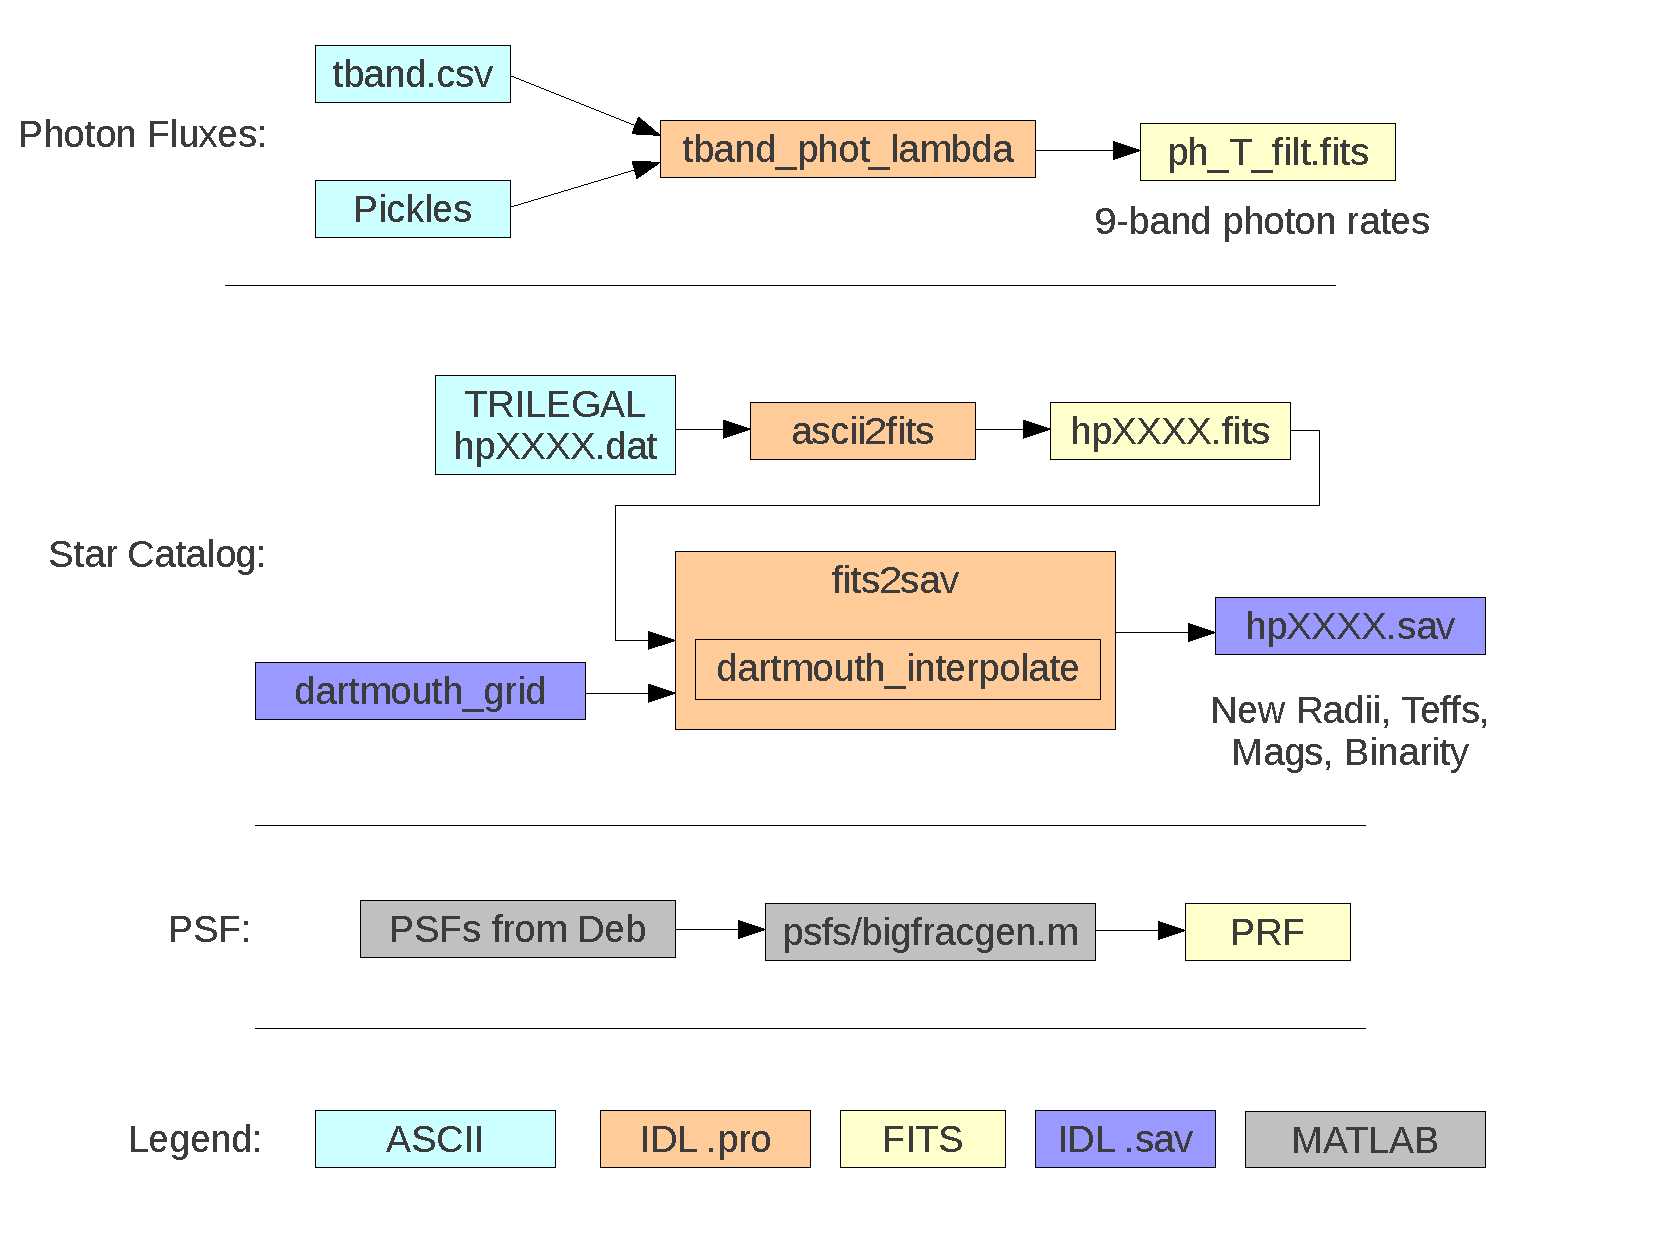
\includegraphics[width=0.9\textwidth]{preprocess.pdf}
\end{center}
\caption{Pre-processing of simulation files. From top to bottom, these routines calculate the photon fluxes, build the star catalog, and integrate the PSF.}
\label{fig:preprocess}
\end{figure}


\subsection{Photon Fluxes}
We divide the TESS bandpass into 9 synthetic filters where we separately calculate the PRF and photon fluxes for a wide range of spectral types. The PRFs are then summed, weighted by the photon fluxes. 
The IDL procedure \texttt{tband\_phot\_lambda.pro} in the \texttt{PhotonFluxes} directory integrates the spectra of stars to calculate the fluxes.

\subsection{Star catalog}
The TRILEGAL catalogs were originally downloaded as ASCII files to the \texttt{~/trilegal} directory. 
To conserve disk space, these were converted to FITS files using \texttt{ascii2fits.pro}, and the original ASCII files were deleted. 
One should not have to re-download or re-convert the TRILEGAL files unless a serious problem is discovered in the input settings, which are documented in the ApJ paper. 

Next, the FITS files are converted to star structures in IDL using \texttt{fits2sav\_wrapper.pro}. This script is called once for each of the three levels of star catalog; magnitude limits and duplication of stars is handled automatically for each file name: \\
\\
\texttt{IDL> fits2sav\_wrapper, `~/trilegal/hp*.fits'}\\
\texttt{IDL> fits2sav\_wrapper, `~/trilegal/bk*.fits'}\\
\texttt{IDL> fits2sav\_wrapper, `~/trilegal/dp*.fits'}\\
\\
The heavy lifting is performed by \texttt{fits2sav.pro}, which enforces the J-band luminosity function, binary statistics, and Dartmouth stellar models.
Running this step over-writes any existing \texttt{.sav} files, but the original FITS files are untouched.
One should not have to run this step unless the stellar properties must be changed.

\subsection{PRF Calculation}
Deb Woods' model of the PSF outputs a MATLAB structure. 
We integrate the PSFs into a PRF using \texttt{bigfracgen.m}; the output is a multi-dimensional FITS file containing the PRF for various wavelengths, field angles, and offsets between the PSF and the pixel boundaries. \textbf{This script must be re-run if the optical model changes.}

The first three lines of \texttt{bigfracgen.m} specify the input structure file name, the output file name, and a flag to turn the spacecraft jitter on or off. 
The integration of the PSF over pixel boundaries is handled by the function \texttt{psfedoff.m}. 

Jittering the PSF makes the computation take much longer since this function re-calculates the PRF from the PSF at different sub-pixel offsets and wavelengths with 2-second sampling. It has very little impact on the planet yield since the RMS jitter is $\sim$1''.

\section{Simulation}
The IDL procedure \texttt{main.pro} runs the simulation. From the command prompt, it can be invoked with \\
\\
\texttt{> idl -e main \&>main.out}\\
\\
where the simulation writes its status to the file \texttt{main.out}. 
All of the detected transiting exoplanets or eclipsing binaries are written to a FITS table; the file name is specified in \texttt{main.pro}.

The only real purpose of \texttt{main.pro} is to call \texttt{tile\_wrapper.pro} and its sub-routines with the most commonly-adjusted parameters as inputs. This protects \texttt{tile\_wrapper.pro} from any operator error. 

The simulation supports several modes. The \texttt{eclass} flags select the kinds of eclipsing systems that are considered, so if one is only interested in transiting planets, the runtime of the simulation can be reduced. If the \texttt{ps\_only} flag is set, only the postage stamps are considered. If the \texttt{detmag} flag is set to a number representing an apparent magnitude, then the simulation considers all transiting or eclipsing systems brighter than this apparent magnitude (in the $V$, $I_C$, or $K$ bands) to be ``detected''. This is useful for quickly generating a magnitude-limited catalog of all eclipsing systems in the sky. Otherwise, the full TESS model is used to determine whether an eclipse is ``detected.''

The hierarchy of the sub-routines called from \texttt{tile\_wrapper.pro} is shown in Figure~\ref{fig:flow}. For each HEALPix tile, \texttt{tile\_wrapper} loads the three TRILEGAL catalogs, adds eclipses, ``observes'' them, and builds the output FITS table of the ``detected'' eclipses. The roles of each major sub-routine is described below, but these should rarely need to be modified.

\subsection{Postage Stamp Selection}
The selection of target stars for postage stamp observations is handled in \texttt{ps\_sel.pro}. As described in the ApJ paper, the target stars are selected based on the detectability of small planets with a fiducial 10-day period. A threshold planet radius of 2.5 $R_{\oplus}$ gives 2$\times 10^5$ target stars. To change the number of target stars, one can simply move the threshold radius up and down. However, the simulation must be run through all of the HEALPix tiles in order to count the total number of target stars, which is reported at the end of the simulation. Since the counting of target stars does not require calling most of the subroutines, I recommend running the simulation with the $\texttt{detmag}$ flag set and only eclipsing binaries selected to minimize the run time. Once the number of target stars is tweaked, the simulation can be run normally. 

\subsection{Sky Coverage}
The number of pointings with which TESS observs each eclipse is computed in \texttt{eclip\_survey.pro}. This routine takes the number of pointings per hemisphere and field-of-view as input parameters.

\subsection{Detection}
The signal-to-noise ratio (SNR) of each eclipse is computed with \texttt{eclip\_observe.pro}. The most computationally-intensive step is calculating the diluting flux from the stars neighboring a transiting or eclipsing system. 
For this reason, the code calculates the SNR twice (with repeated calls of \texttt{calc\_noise\_eclip.pro}) before the calculation of diluting flux and after. Only the systems with a sufficiently high SNR on the first round have the diluting flux calculated, and only the systems with a sufficiently high SNR with the diluting flux survive to be reported by the simulation.

This routine also calls \texttt{calc\_noise\_cen.pro} to calculate the centroid shifts and centroid uncertainties from the PRF images.

The dilution routines are \texttt{dilute\_eclipse\_img.pro}, \texttt{dilute\_beb.pro}, and \texttt{dilute\_binary.pro}. 
These are all similar routines, but they calculate the dilution of an eclipse from different sources. 
\texttt{dilute\_eclipse\_img.pro} dilutes a target star with unassociated neighboring stars drawn at random from the star catalogs.
\texttt{dilute\_beb.pro} dilutes BEBs and HEBs with the flux of the target star. 
Finally, \texttt{dilute\_binary.pro} dilutes target stars with planets or BEBs with the binary companion of the target star.

\begin{figure}
\begin{center}
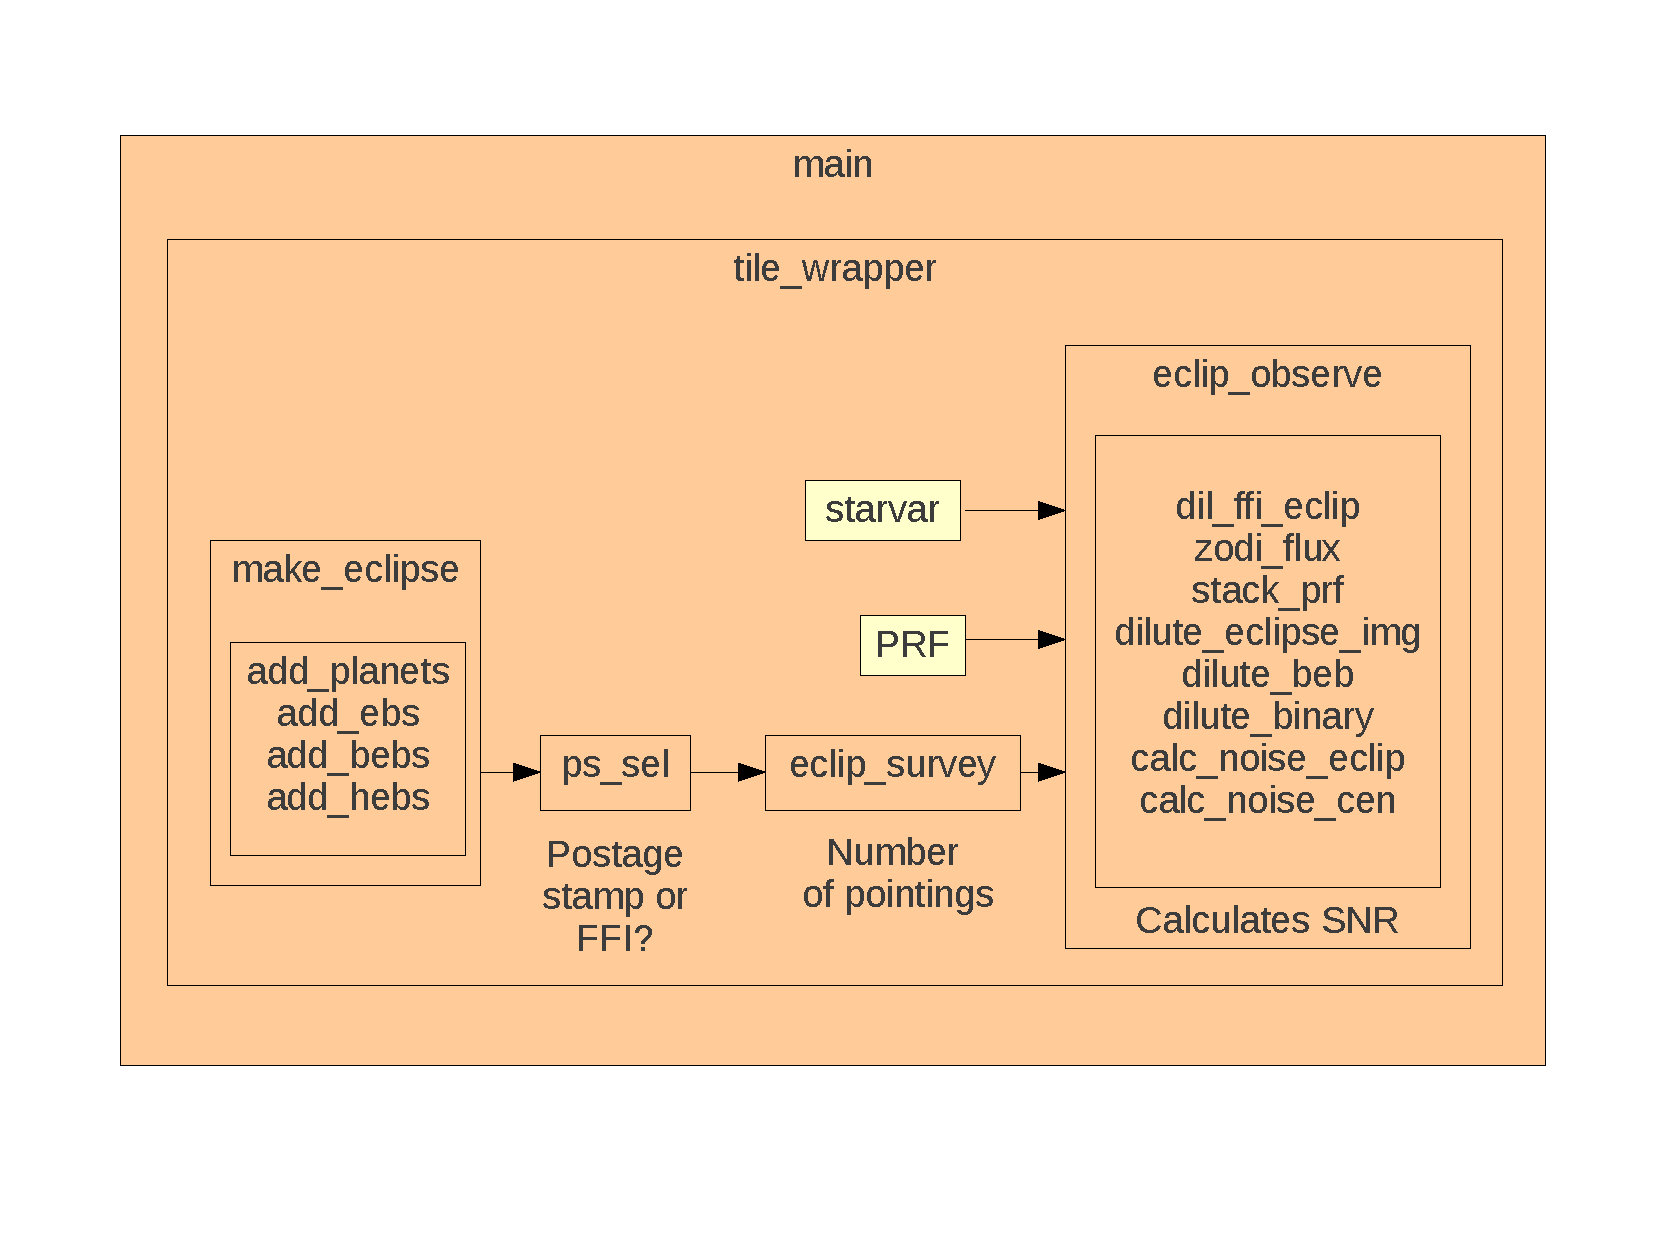
\includegraphics[width=0.9\textwidth]{flow.pdf}
\end{center}
\caption{Structure of the simulation code. The user generally interacts with \texttt{main.pro}, but some adjustments can only be made through the sub-routines.}
\label{fig:flow}
\end{figure}

\section{Post-Processing}
The analysis and visualization of the simulation output is exclusively done in MATLAB. The scripts are located in the \texttt{Paper} directory.

The first step is to load the output FITS file from the simulation. This is done with \texttt{unpack.m}; the first line of this script specifies the file. This script also finds the number of planets detected in several classes (Earths, Super-Earths, Neptunes, HZ, etc.). If multiple trials are run (with the \texttt{n\_trial} parameter in \texttt{main.pro}), then the mean number of planets for each class are calculated.

After the simulation is loaded into MATLAB, any of the scrips used to generate the figures in the ApJ paper can be run. 
The most useful for systems engineering purposes is probably \texttt{plot\_yield.m}, which re-makes the bar plot of planet and false-positive yields. The script \texttt{fp.m} computes the number of false-positives and the fractions that can be identified in the TESS photometry.


%\begin{deluxetable}{lcccc}
%
%\tabletypesize{\scriptsize}
%\tablecolumns{5}
%\tablewidth{0pt}
%\tablecaption{Resolution-limited $I$ magnitudes\label{tbl:m_lim}}
%
%\tablehead{
%\colhead{$b$~[deg]} &
%\colhead{$l=0^\circ$} &
%\colhead{$l=60^\circ$} &
%\colhead{$l=120^\circ$} &
%\colhead{$l=180^\circ$}
%}
%
%\startdata
%    0 &  13.10 &  14.00 &  15.07 &  15.44 \\
%   10 &  14.21 &  15.23 &  15.85 &  16.56 \\
%   20 &  15.93 &  16.79 &  17.52 &  18.32 \\
%   30 &  17.28 &  18.22 &  19.25 &  19.96 \\
%   40 &  18.46 &  19.49 &  20.56 &  21.25
%\enddata
%
%\end{deluxetable}

\end{document}

\begin{thebibliography}{}

\end{thebibliography}

\end{document}

